\section{Lezione 17 24/10/2023}

\subsection{Grafi}
I grafi sono una coppia di insiemi definita come:(V,E) (chiamato oggetto), dove V e un insieme finito di elementi che compongono il grafo chiamati \textbf{vertici}. L'insieme E rappresenta l'insieme degli \textbf{archi}.

L'insieme E e costituito da una coppia composta cosi definita: $E \subseteq V x V$, quindi una coppia formata da due vertici dell'insieme \textbf{V}.

L'insieme E e in relazione simmetrica. 

I  grafi non posseggono foglie, ma esistono grafi con archi uscenti soltanto, verso nodi che non hanno altri collegamenti.

Un grafo si dice \textbf{completo} quando il suo numero di archi e uguale a n.

\begin{figure}[H]
	\begin{center}
		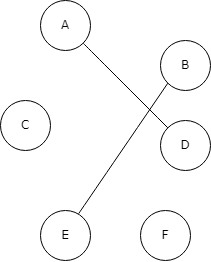
\includegraphics[width=0.2\textwidth]{grafo_orientato}
	\end{center}
\end{figure}
$$ V = \{A,B,C,D,E,F\} $$
$$E = \{(A,D), (B,E)\}$$





\subsection{Grafo Orientato}
Un grafo orientato e un grafo che ha gli archi direzionati, cioe che vanno da una direzione all'altra, solitamente nella rappresentazione grafica a coppie, la direzione va dal primo elemento verso il secondo.

(I secondi elementi nella coppia sono i cosiddetti "Carrier della relazione").

\begin{figure}[H]
	\begin{center}
		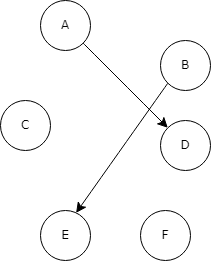
\includegraphics[width=0.2\textwidth]{grafo_non_orientato}
	\end{center}
\end{figure}

Per "tornare" al caso in cui il grafo non e orientato, bisogna avere aggiungere degli archi orientati nel verso opposto a quelli che gia esistono:

\begin{figure}[H]
	\begin{center}
		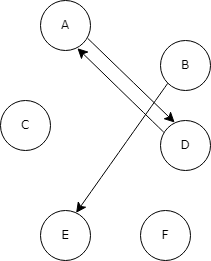
\includegraphics[width=0.2\textwidth]{grafo_non_orientato_doppio}
	\end{center}
\end{figure}


\subsection{Alberi e Grafi}

Gli alberi sono particolari tipi di grafi dove la relazione che vige tra i nodi e quella di parentela (padre figli). In esso i tragitti non sono infiniti come possono essere in un grafo.
Un grafo non puo essere ricostruito come un albero nel caso in cui un nodo si perde, poiche non sappiamo quanti e quali archi abbia perso a differenza di un nodo di un albero che puo avere un solo padre e uno o 2 figli.

\subsection{Grafi Pesati}
I grafi pesati sono un'applicazione dei grafi ordinati e non, dove ad ogni arco viene associato un numero (peso).

\subsection{Grado di un Vertice}

Il grado di un vertice puo dividersi in 
\begin{itemize}
	\item Grado entrante, cioe il numero di archi che entrano nell'arco
	\item Grado uscente, cioe il numero di archi che escono dall'arco
\end{itemize}

P.S. un cappio e un arco che esce e entra nello stesso nodo.
%immagine

Ogni vertice puo avere come massimo numero di archi (entranti e uscenti), il numero di vertici del grafo.
$$n = |V|$$

\subsection{Percorsi}
Sia $v,w \in V$ e definito $\pi$ = il percorso da $v \text{in} w$ nel grafo G. Per percorso si intende la sequenza di vertici che si impegnano per arrivare al vertice stabilito. 

$$\pi = v_0,v_1,v_2,\dots,v_k$$ tale che 

\begin{itemize}
	\item $v_0$ = $u$
	\item $v_k$ = $v$
	\item $\forall  0\le i \le k-1 = (v_i,v_{i+1})$
\end{itemize}

La coppia di valori tali che il secondo e il successivo del primo.

\subsection{Raggiungibilita di un nodo}

Un nodo $v $ e detto raggiungibile da $u$ un un grafico $G \iff \exists \pi | \pi \text{e un percorso da }u \text{in } v$.

Quindi solo se esiste un percorso (insieme di nodi raggiungibili attraverso degli archi) da u in v.

La raggiungibilita puo essere scritta come funzione $\text{Reach} \in V x V$. La funzione Reach possiede delle proprieta:
\begin{itemize}
	\item Riflessiva
			$v \text{ e raggiungibile da } v$ poiche $(v,v)$ e una coppia $\in E$, ed e chiamato percorso senza archi. 
	\item Transitiva
			Se $(u,z) \in Reach$ e $(z,v) \in Reach$ allora avremo che sicuramente $(u,v) \in Reach$.
			Se esiste un percorso che da $u$ va in $z$ e da $z$ in $v$, allora esistera un percorso che raggiunge $(u,z)$, concatenando i percorsi dei due.
\end{itemize}  

\subsection{Percorsi Ciclici}
Un grafo orientato in cui non esistono cicli semplici e detto \textbf{Grafo Ciclico}, dove per ciclo semplice si intende una "ripetizione di un vertice in una sequenza".

%foto

\subsection{Sottografo}
Dato $G = (V,E)$, allora $G^{\prime} = (V^{\prime},E^{\prime})$ e detto sottografo di $G$.
La condizione principale per far si che $G^{\prime}$ sia sottografo e che $V^{\prime} \in V$.
In questo caso il numero degli archi e : $E^{\prime} \in E \cap (V^{\prime} x V^{\prime})$.
Nel caso in cui $E^{\prime} = E$, allora ci troviamo in un \textbf{sottografo indotto}.



